\section{(W) Space Discretization - Avoidance Grid}\label{s:AvoidanceGrid}
    \noindent UAS operates in some space which is given:
    \begin{itemize}
        \item Sensor ranges
        \item UAS maneuverability
        \item Computation power
        \item Airworthiness requirements (IFR/VFR)
        \item intended reaction times for event-bases/emergency situations
    \end{itemize}
    \noindent In this section discuss:
    \begin{itemize}
    	\item Proposed clustering method near thick, far loose , \cite{zaiane2002clustering}.
        \item Polar grid vs Euclidian homogenous grid
        \item Trajectory intersection (mixed-integer) problem
        \item Avoidance grid scaling based on previously mentioned factors
        \item Space (cell) properties:
        \begin{itemize}
            \item Visibility - how is space visible
            \item Occupancy - is space occupied/free ?
            \item Reachibility - is there safe way to given point ?
        \end{itemize}
    \end{itemize}
    \begin{figure}[H]
        \centering
        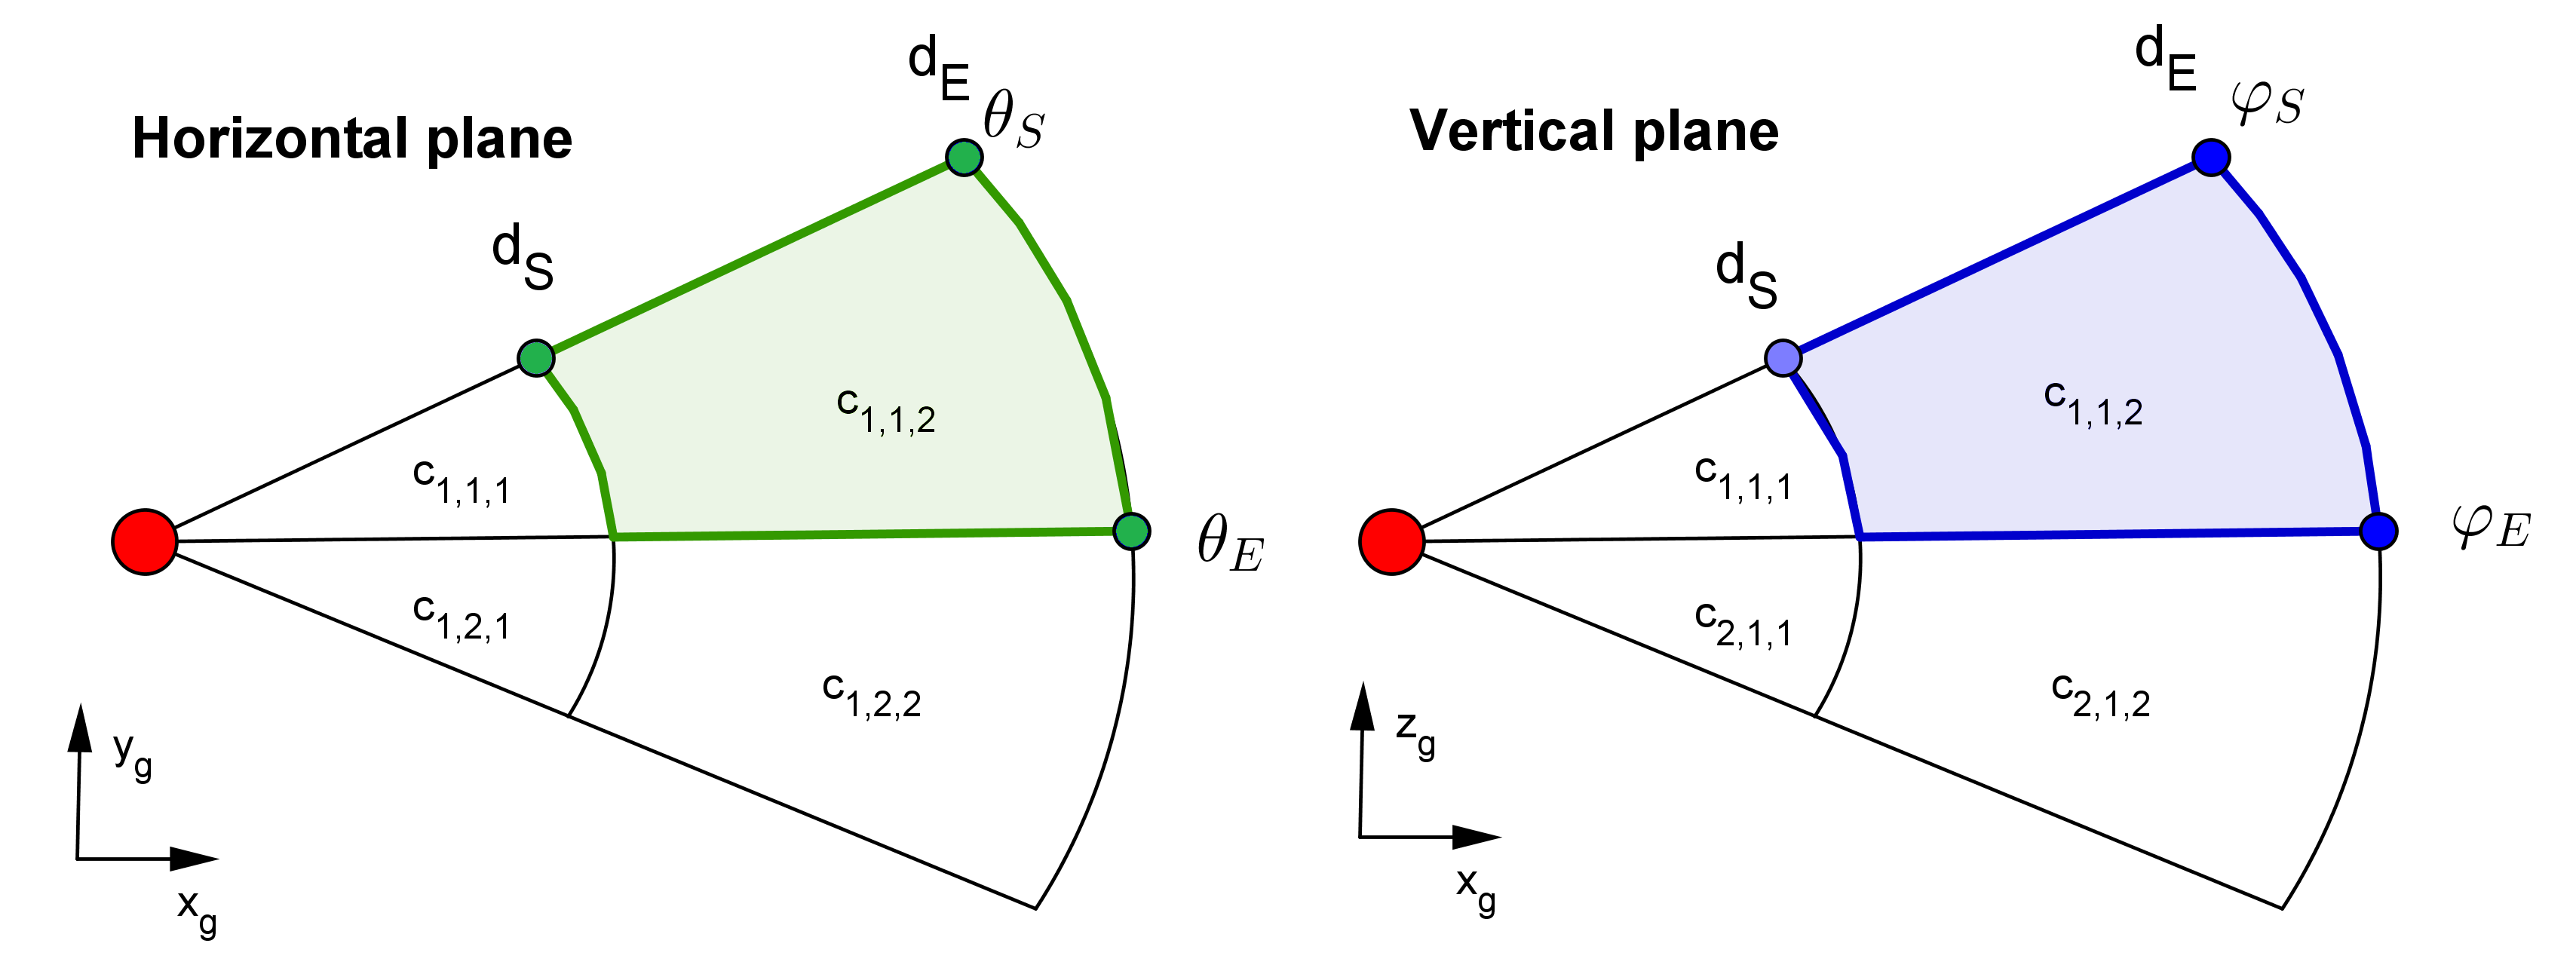
\includegraphics[width=0.80\linewidth]{\FIGDIR/TE020AvoidanceOrVisibilityGridCellExample} 
        \caption{\emph{Cell} of \emph{Avoidance Grid} with \emph{Boundaries}.}
        \label{fig:cellBoundariesInAvoidanceGrid}
    \end{figure}
